\documentclass[tikz,border=10pt]{standalone}
\usepackage{tikz}
\usepackage{amsmath,amssymb}
\usepackage{fontawesome5}
\usetikzlibrary{arrows.meta,positioning,fit,backgrounds,calc,shadows,shapes.geometric}

% Color definitions
\definecolor{lavenderDark}{RGB}{15, 44, 89}
\definecolor{lavenderDeep}{RGB}{10, 28, 58}
\definecolor{lavenderMedium}{RGB}{29, 78, 158}
\definecolor{lavenderLight}{RGB}{240, 246, 255}
\definecolor{lavenderBorder}{RGB}{180, 205, 237}
\definecolor{prismNavy}{RGB}{15, 44, 89}
\definecolor{prismBlue}{RGB}{29, 78, 158}
\definecolor{prismTeal}{RGB}{13, 148, 136}
\definecolor{prismGold}{RGB}{217, 119, 6}
\definecolor{prismDark}{RGB}{15, 23, 42}
\definecolor{cInput}{RGB}{241, 245, 249}
\definecolor{cStem}{RGB}{224, 242, 254}
\definecolor{cStage1}{RGB}{209, 250, 229}
\definecolor{cStage2}{RGB}{254, 243, 199}
\definecolor{cStage4}{RGB}{207, 250, 254}
\definecolor{cHead}{RGB}{219, 234, 254}

\begin{document}
% Level-1 Data Flow Diagram (DFD) for Blockchain Electronic Voting System
\begin{tikzpicture}[
  x=1.0cm, y=1.0cm,
  entity/.style={
    rectangle, draw=lavenderDark!90, line width=1.1pt, rounded corners=4pt,
    align=center, inner sep=5pt, font=\fontsize{8.5}{10.5}\selectfont\bfseries,
    text width=3.0cm, fill=cInput, drop shadow={opacity=0.12}
  },
  store/.style={
    rectangle, draw=lavenderDark!85, line width=1.1pt, rounded corners=2pt,
    align=center, inner sep=4.5pt, font=\fontsize{8.0}{9.5}\selectfont,
    text width=3.3cm, fill=lavenderLight, drop shadow={opacity=0.10}
  },
  proc/.style={
    circle, draw=lavenderMedium!95, line width=1.1pt,
    align=center, inner sep=2pt, minimum size=2.20cm,
    font=\fontsize{8.0}{9.5}\selectfont\bfseries, fill=cStage1, drop shadow={opacity=0.10}
  },
  procblue/.style={proc, fill=cStage4},
  procgold/.style={proc, fill=cStage2},
  prochead/.style={proc, fill=cHead},
  dfdarr/.style={
    -{Stealth[scale=1.0, length=5pt, width=4pt]}, line width=1.0pt, draw=lavenderDark!90
  },
  flowlbl/.style={
    font=\fontsize{7.2}{8.5}\selectfont\bfseries, fill=white, inner sep=2.0pt,
    rounded corners=2pt, text=lavenderDark, draw=lavenderBorder!70, line width=0.45pt,
    align=center
  }
]

  % External Entities (Left column and Right column)
  \node[entity] (admin) at (-7.2, 2.7) {\faUserShield\ Election\\[2pt]Administrator};
  \node[entity, fill=cStem!75] (voter) at (-7.2, -2.6) {\faUser\ Registered\\[2pt]Voter (MetaMask)};
  \node[entity, fill=cInput!70] (auditor) at (9.4, 0.0) {\faEye\ Public Auditor /\\[2pt]Observer};

  % Processes (Column 2: p1, p2; Column 3: p4, p3; Column 4: p5)
  \node[prochead] (p1) at (-2.9, 2.7) {1.0\\[1pt]Whitelist\\[1pt]\& Setup};
  \node[procblue] (p2) at (-2.9, -2.6) {2.0\\[1pt]Wallet Auth\\[1pt]\& Connect};
  \node[procgold] (p3) at (1.6, -2.6) {3.0\\[1pt]Cast Ballot\\[1pt]Transaction};
  \node[proc] (p4) at (1.6, 2.7) {4.0\\[1pt]Double-Vote\\[1pt]Mitigation};
  \node[prochead] (p5) at (5.2, 0.0) {5.0\\[1pt]Consensus\\[1pt]\& Tally};

  % Data Stores
  \node[store] (d1) at (-0.7, 0.0) {\textbf{D1: Voter Mapping}\\[2pt]\scriptsize \texttt{voters[address]}};
  \node[store] (d2) at (1.6, 4.9) {\textbf{D2: Candidates}\\[2pt]\scriptsize \texttt{candidates[]}};
  \node[store] (d3) at (5.2, -2.8) {\textbf{D3: Blockchain Ledger}\\[2pt]\scriptsize Immutable Blocks \& Receipts};

  % Admin Flows
  \draw[dfdarr] (admin) -- node[above=2pt, flowlbl] {Voter\\Addresses} (p1);
  \draw[dfdarr] (admin.north) |- node[pos=0.72, above=2pt, flowlbl] {Candidate Monikers} (d2.west);
  \draw[dfdarr] (p1.south) to[out=285, in=125] node[pos=0.48, left=3pt, flowlbl] {Register\\Flag} (d1.north west);

  % Voter Flows
  \draw[dfdarr] (voter) -- node[above=2pt, flowlbl] {Connect\\Request} (p2);
  \draw[dfdarr] (p2.north) to[out=75, in=235] node[pos=0.48, left=3pt, flowlbl] {Query\\Status} (d1.south west);
  \draw[dfdarr] (p2) -- node[above=2pt, flowlbl] {Address OK} (p3);
  \draw[dfdarr] (p3) -- node[pos=0.50, right=3pt, flowlbl] {Signed Tx} (p4);

  % Double-Vote Mitigation & Candidate Flows
  \draw[dfdarr] (p4.south west) to[out=230, in=50] node[pos=0.50, above left=1pt, flowlbl] {Atomic\\Check} (d1.north east);
  \draw[dfdarr] (p4) -- node[right=3pt, flowlbl] {Inc Count} (d2);
  \draw[dfdarr] (p4.south east) to[out=320, in=115] node[pos=0.48, above right=1pt, flowlbl] {Approved\\Vote} (p5.north);

  % Consensus & Public Audit Flows
  \draw[dfdarr] (p5) -- node[right=3pt, flowlbl] {Commit\\Block} (d3);
  \draw[dfdarr] (p5) -- node[above=2pt, flowlbl] {Real-Time\\Results} (auditor);
  \draw[dfdarr] (d3.east) -| node[pos=0.35, right=3pt, flowlbl] {Audit Trails} (auditor.south);

\end{tikzpicture}
\end{document}
